
%__________________
\section{One-sample means with the $t$ distribution}
\label{oneSampleMeansWithTDistribution}

\subsection[Nearly normal population with known SD]{Nearly normal population with known SD (special topic)}
\label{nearlyNormalPopWithKnownSD}

\index{Central Limit Theorem!normal data|(}

In rare circumstances we know important characteristics of a population. For instance, we might know a population is nearly normal and we may also know its parameter values. Even so, we may still like to study characteristics of a random sample from the population. Consider the conditions required for modeling a sample mean using the normal distribution:
\begin{enumerate}
\setlength{\itemsep}{0mm}
\item[(1)] The observations are independent.
\item[(2)] The sample size $n$ is at least 30.
\item[(3)] The data distribution is not strongly skewed.
\end{enumerate}
These conditions are required so we can adequately estimate the standard deviation and so we can ensure the distribution of sample means is nearly normal. However, if the population is known to be nearly normal, the sample mean is always nearly normal (this is a special case of the Central Limit Theorem). If the standard deviation is also known, then conditions (2) and (3) are not necessary for those data.

\begin{example}{The heights of male seniors in high school closely follow a normal distribution $N(\mu=70.43, \sigma=2.73)$, where the units are inches.\footnote{These values were computed using the USDA Food Commodity Intake Database.} If we randomly sampled the heights of five male seniors, what distribution should the sample mean follow?}\label{simpleSampleOfFiveMaleSeniors}
The population is nearly normal, the population standard deviation is known, and the heights represent a random sample from a much larger population, satisfying the independence condition. Therefore the sample mean of the heights will follow a nearly normal distribution with mean $\mu=70.43$ inches and standard error $SE=\sigma/\sqrt{n} = 2.73/\sqrt{5}=1.22$ inches.
\end{example}

\begin{termBox}{\tBoxTitle{Alternative conditions for applying the normal distribution to model the sample mean}
If the population of cases is known to be nearly normal and the population standard deviation $\sigma$ is known, then the sample mean $\bar{x}$ will follow a nearly normal distribution $N(\mu, \sigma/\sqrt{n})$ if the sampled observations are also independent.}
\end{termBox}

Sometimes the mean changes over time but the standard deviation remains the same. In such cases, a sample mean of small but nearly normal observations paired with a known standard deviation can be used to produce a confidence interval for the current population mean using the normal distribution.

\begin{example}{Is there a connection between height and popularity in high school? Many students may suspect as much, but what do the data say? Suppose the top 5 nominees for prom king at a high school have an average height of 71.8 inches. Does this provide strong evidence that these seniors' heights are not representative of all male seniors at their high school?}
If these five seniors are height-representative, then their heights should be like a random sample from the distribution given in Example~\ref{simpleSampleOfFiveMaleSeniors}, $N\left(\mu=70.43, \sigma = 2.73\right)$, and the sample mean should follow $N\left(\mu=70.43, \sigma/\sqrt{n} = 1.22\right)$. Formally we are conducting what is called a \emph{hypothesis test}, which we will discuss in greater detail during the next section. We are weighing two possibilities:
\begin{itemize}
\setlength{\itemsep}{0mm}
\item[$H_0$:] The prom king nominee heights are representative; $\bar{x}$ will follow a normal distribution with mean 70.43 inches and standard error 1.22 inches.
\item[$H_A$:] The heights are not representative; we suspect the mean height is different from 70.43 inches.
\end{itemize}
If there is strong evidence that the sample mean is not from the normal distribution provided in $H_0$, then that suggests the heights of prom king nominees are not a simple random sample (i.e. $H_A$ is true). We can look at the Z score of the sample mean to tell us how unusual our sample is. If $H_0$ is true:
\begin{align*}
Z = \frac{\bar{x} - \mu}{\sigma/\sqrt{n}} = \frac{71.8 - 70.43}{1.22} = 1.12
\end{align*}
A Z score of just 1.12 is not very unusual (we typically use a threshold of $\pm2$ to decide what is unusual), so there is not strong evidence against the claim that the heights are representative. This does not mean the heights are actually representative, only that this very small sample does not necessarily show otherwise.
\end{example}

\begin{tipBox}{\tipBoxTitle{Relaxing the nearly normal condition}
As the sample size becomes larger, it is reasonable to \emph{slowly} relax the nearly normal assumption on the data when dealing with small samples. By the time the sample size reaches 30, the data must show strong skew for us to be concerned about the normality of the sampling distribution.}
\index{Central Limit Theorem!normal data|)}
\end{tipBox}

The motivation in Chapter~\ref{foundationsForInference} for requiring a large sample was two-fold. First, a large sample ensures that the sampling distribution of $\bar{x}$ is nearly normal. We will see in Section~\ref{normalityCond} that if the population data are nearly normal, then $\bar{x}$ is also nearly normal regardless of the sample size. The second motivation for a large sample was that we get a better estimate of the standard error when using a large sample. The standard error estimate will not generally be accurate for smaller sample sizes, and this motivates the introduction of the $t$ distribution, which we introduce in Section~\ref{introducingTheTDistribution}.

We will see that the $t$ distribution is a helpful substitute for the normal distribution when we model a sample mean $\bar{x}$ that comes from a small sample. While we emphasize the use of the $t$ distribution for small samples, this distribution may also be used for means from large samples.

\subsection{The normality condition}
\label{normalityCond}

We use a special case of the Central Limit Theorem to ensure the distribution of the sample means will be nearly normal, regardless of sample size, provided the data come from a nearly normal distribution.

\begin{termBox}{\tBoxTitle{Central Limit Theorem for normal data}
The sampling distribution of the mean is nearly normal when the sample observations are independent and come from a nearly normal distribution. This is true for any sample size.
\index{Central Limit Theorem!normal data|)}}
\end{termBox}

While this seems like a very helpful special case, there is one small problem. It is inherently difficult to verify normality in small data sets.

\begin{caution}
{Checking the normality condition}
{We should exercise caution when verifying the normality condition for small samples. It is important to not only examine the data but also think about where the data come from. For example, ask: would I expect this distribution to be symmetric, and am I confident that outliers are rare?}
\end{caution}

You may relax the normality condition as the sample size goes up. If the sample size is~10 or more, slight skew is not problematic. Once the sample size hits about~30, then moderate skew is reasonable. Data with strong skew or outliers require a more cautious analysis.


\subsection{Introducing the $t$ distribution}
\label{introducingTheTDistribution}

\index{$t$ distribution|(}

The second reason we previously required a large sample size was so that we could accurately estimate the standard error using the sample data. In the cases where we will use a small sample to calculate the standard error, it will be useful to rely on a new distribution for inference calculations: the $t$ distribution. A $t$ distribution, shown as a solid line in Figure~\ref{tDistCompareToNormalDist}, has a bell shape. However, its tails are thicker than the normal model's. This means observations are more likely to fall beyond two standard deviations from the mean than under the normal distribution.\footnote{The standard deviation of the $t$ distribution is actually a little more than 1. However, it is useful to always think of the $t$ distribution as having a standard deviation of 1 in all of our applications.} These extra thick tails are exactly the correction we need to resolve the problem of a poorly estimated standard error.

\begin{figure}
\centering
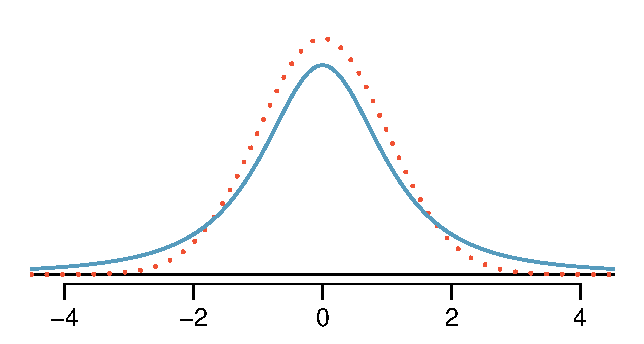
\includegraphics[height=45mm]{05/figures/tDistCompareToNormalDist/tDistCompareToNormalDist}
\caption{Comparison of a $t$ distribution (solid line) and a normal distribution (dotted line).}
\label{tDistCompareToNormalDist}
\end{figure}

The $t$ distribution, always centered at zero, has a single parameter: degrees of freedom. The \termsub{degrees of freedom (df)}{degrees of freedom (df)!$t$ distribution} describe the precise form of the bell-shaped $t$ distribution. Several $t$ distributions are shown in Figure~\ref{tDistConvergeToNormalDist}. When there are more degrees of freedom, the $t$~distribution looks very much like the standard normal distribution.

\begin{figure}
\centering
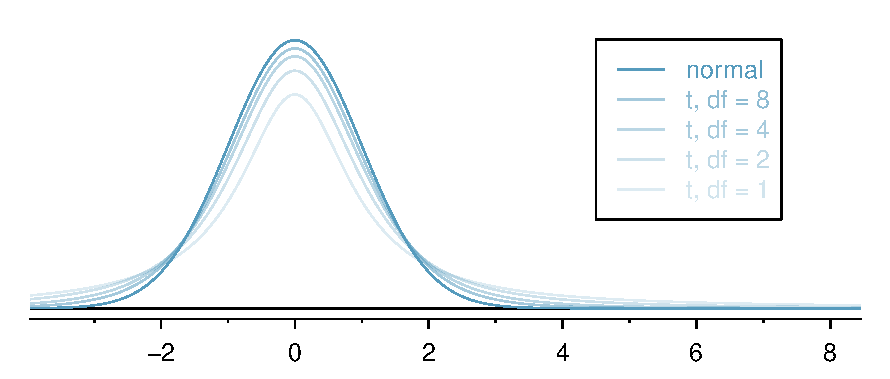
\includegraphics[width=0.8\textwidth]{05/figures/tDistConvergeToNormalDist/tDistConvergeToNormalDist}
\caption{The larger the degrees of freedom, the more closely the $t$ distribution resembles the standard normal model.}
\label{tDistConvergeToNormalDist}
\end{figure}

\begin{termBox}{\tBoxTitle{Degrees of freedom (df)}
The degrees of freedom describe the shape of the $t$ distribution. The larger the degrees of freedom, the more closely the distribution approximates the normal model.}
\end{termBox}

When the degrees of freedom is about 30 or more, the $t$ distribution is nearly indistinguishable from the normal distribution. In Section~\ref{tDistSolutionToSEProblem}, we relate degrees of freedom to sample size.

We will find it very useful to become familiar with the $t$ distribution, because it plays a very similar role to the normal distribution during inference for small samples of numerical data. We use a \term{t table}, partially shown in Table~\ref{tTableSample}, in place of the normal probability table for small sample numerical data. A larger table is presented in Appendix~\vref{tDistributionTable}.

\begin{table}[hht]
\centering
\begin{tabular}{r | rrr rr}
one tail & \hspace{1.5mm}  0.100 & \hspace{1.5mm} 0.050 & \hspace{1.5mm} 0.025 & \hspace{1.5mm} 0.010 & \hspace{1.5mm} 0.005  \\
two tails & 0.200 & 0.100 & 0.050 & 0.020 & 0.010 \\
\hline
{$df$} \hfill 1  &  {\normalsize  3.08} & {\normalsize  6.31} & {\normalsize 12.71} & {\normalsize 31.82} & {\normalsize 63.66}  \\ 
2  &  {\normalsize  1.89} & {\normalsize  2.92} & {\normalsize  4.30} & {\normalsize  6.96} & {\normalsize  9.92}  \\ 
3  &  {\normalsize  1.64} & {\normalsize  2.35} & {\normalsize  3.18} & {\normalsize  4.54} & {\normalsize  5.84}  \\ 
$\vdots$ & $\vdots$ &$\vdots$ &$\vdots$ &$\vdots$ & \\
17  &  {\normalsize  1.33} & {\normalsize  1.74} & {\normalsize  2.11} & {\normalsize  2.57} & {\normalsize  2.90}  \\ 
\highlightO{18}  &  \highlightO{\normalsize  1.33} & \highlightO{\normalsize  1.73} & \highlightO{\normalsize  2.10} & \highlightO{\normalsize  2.55} & \highlightO{\normalsize  2.88}  \\ 
19  &  {\normalsize  1.33} & {\normalsize  1.73} & {\normalsize  2.09} & {\normalsize  2.54} & {\normalsize  2.86}  \\ 
20  &  {\normalsize  1.33} & {\normalsize  1.72} & {\normalsize  2.09} & {\normalsize  2.53} & {\normalsize  2.85}  \\ 
$\vdots$ & $\vdots$ &$\vdots$ &$\vdots$ &$\vdots$ & \\
400  &  {\normalsize  1.28} & {\normalsize  1.65} & {\normalsize  1.97} & {\normalsize  2.34} & {\normalsize  2.59}  \\ 
500  &  {\normalsize  1.28} & {\normalsize  1.65} & {\normalsize  1.96} & {\normalsize  2.33} & {\normalsize  2.59}  \\ 
$\infty$  &  {\normalsize  1.28} & {\normalsize  1.64} & {\normalsize  1.96} & {\normalsize  2.33} & {\normalsize  2.58}  \\ 
\end{tabular}
\caption{An abbreviated look at the $t$ table. Each row represents a different $t$ distribution. The columns describe the cutoffs for specific tail areas. The row with $df=18$ has been \highlightO{highlighted}.}
\label{tTableSample}
\end{table}

Each row in the $t$ table represents a $t$ distribution with different degrees of freedom. The columns correspond to tail probabilities. For instance, if we know we are working with the $t$ distribution with $df=18$, we can examine row 18, which is \highlightO{highlighted} in Table~\ref{tTableSample}. If we want the value in this row that identifies the cutoff for an upper tail of 10\%, we can look in the column where \emph{one tail} is 0.100. This cutoff is 1.33. If we had wanted the cutoff for the lower 10\%, we would use -1.33. Just like the normal distribution, all $t$ distributions are symmetric.

\begin{example}{What proportion of the $t$ distribution with 18 degrees of freedom falls below -2.10?}
Just like a normal probability problem, we first draw the picture in Figure~\ref{tDistDF18LeftTail2Point10} and shade the area below -2.10. To find this area, we identify the appropriate row: $df=18$. Then we identify the column containing the absolute value of -2.10; it is the third column. Because we are looking for just one tail, we examine the top line of the table, which shows that a one tail area for a value in the third row corresponds to 0.025. About 2.5\% of the distribution falls below -2.10. In the next example we encounter a case where the exact $t$ value is not listed in the table.
\end{example}

\begin{figure}
\centering
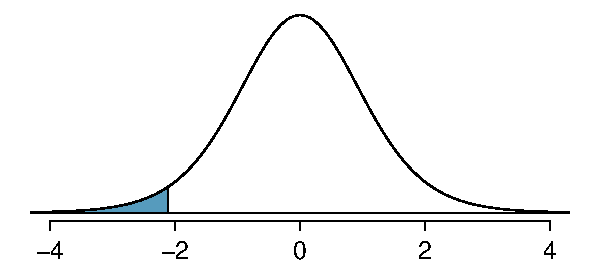
\includegraphics[width=0.55\textwidth]{05/figures/tDistDF18LeftTail2Point10/tDistDF18LeftTail2Point10}
\caption{The $t$ distribution with 18 degrees of freedom. The area below -2.10 has been shaded.}
\label{tDistDF18LeftTail2Point10}
\end{figure}

\textB{\pagebreak}

\begin{example}{A $t$ distribution with 20 degrees of freedom is shown in the left panel of Figure~\ref{tDistDF20RightTail1Point65}. Estimate the proportion of the distribution falling above 1.65.}
We identify the row in the $t$ table using the degrees of freedom: $df=20$. Then we look for 1.65; it is not listed. It falls between the first and second columns. Since these values bound 1.65, their tail areas will bound the tail area corresponding to 1.65. We identify the one tail area of the first and second columns, 0.050 and 0.10, and we conclude that between 5\% and 10\% of the distribution is more than 1.65 standard deviations above the mean. If we like, we can identify the precise area using statistical software: 0.0573.
\end{example}

\begin{figure}
\centering
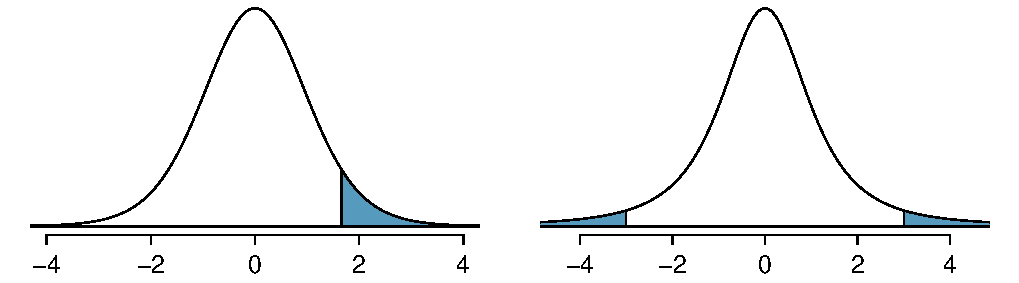
\includegraphics[width=0.85\textwidth]{05/figures/tDistDF20RightTail1Point65/tDistDF20RightTail1Point65}
\caption{Left: The $t$ distribution with 20 degrees of freedom, with the area above 1.65 shaded. Right: The $t$ distribution with 2 degrees of freedom, with the area further than 3 units from 0 shaded.}
\label{tDistDF20RightTail1Point65}
\end{figure}

\begin{example}{A $t$ distribution with 2 degrees of freedom is shown in the right panel of Figure~\ref{tDistDF20RightTail1Point65}. Estimate the proportion of the distribution falling more than 3 units from the mean (above or below).}
As before, first identify the appropriate row: $df=2$. Next, find the columns that capture 3; because $2.92 < 3 < 4.30$, we use the second and third columns. Finally, we find bounds for the tail areas by looking at the two tail values: 0.05 and 0.10. We use the two tail values because we are looking for two (symmetric) tails.
\end{example}

\begin{exercise}
What proportion of the $t$ distribution with 19 degrees of freedom falls above -1.79 units?\footnote{We find the shaded area \emph{above} -1.79 (we leave the picture to you). The small left tail is between 0.025 and 0.05, so the larger upper region must have an area between 0.95 and 0.975.}

\index{$t$ distribution|)}

\end{exercise}



%\subsection{The $t$ distribution as a solution to the standard error problem}
\subsection{The $t$ distribution and the standard error of a mean}
\label{tDistSolutionToSEProblem}

When estimating the mean and standard error from a small sample, the $t$ distribution is a more accurate tool than the normal model. This is true for both small and large samples.

\begin{tipBox}{\tipBoxTitle{When to use the $t$ distribution}
Use the $t$ distribution for inference of the sample mean when observations are independent and nearly normal. You may relax the nearly normal condition as the sample size increases. For example, the data distribution may be moderately skewed when the sample size is at least~30.
}
\end{tipBox}

\index{data!dolphins and mercury|(}

To proceed with the $t$ distribution for inference about a single mean, we must check two conditions.
\begin{description}
\item[Independence of observations.] We verify this condition just as we did before. We collect a simple random sample from less than 10\% of the population, or if it was an experiment or random process, we carefully check to the best of our abilities that the observations were independent.
\item[Observations come from a nearly normal distribution.] This second condition is difficult to verify with small data sets. We often (i) take a look at a plot of the data for obvious departures from the normal model, and (ii) consider whether any previous experiences alert us that the data may not be nearly normal.
\end{description}
When examining a sample mean and estimated standard error from a sample of $n$ independent and nearly normal observations, we use a $t$ distribution with $n-1$ degrees of freedom~($df$). For example, if the sample size was 19, then we would use the $t$ distribution with $df=19-1=18$ degrees of freedom and proceed exactly as we did in Chapter~\ref{foundationsForInference}, except that \emph{now we use the $t$ table}.


\subsection{One sample $t$ confidence intervals}
\label{oneSampleTConfidenceIntervals}

Dolphins are at the top of the oceanic food chain, which causes dangerous substances such as mercury to concentrate in their organs and muscles. This is an important problem for both dolphins and other animals, like humans, who occasionally eat them. For instance, this is particularly relevant in Japan where school meals have included dolphin at times.
\setlength{\captionwidth}{71.5mm}

\begin{figure}[h]
\centering
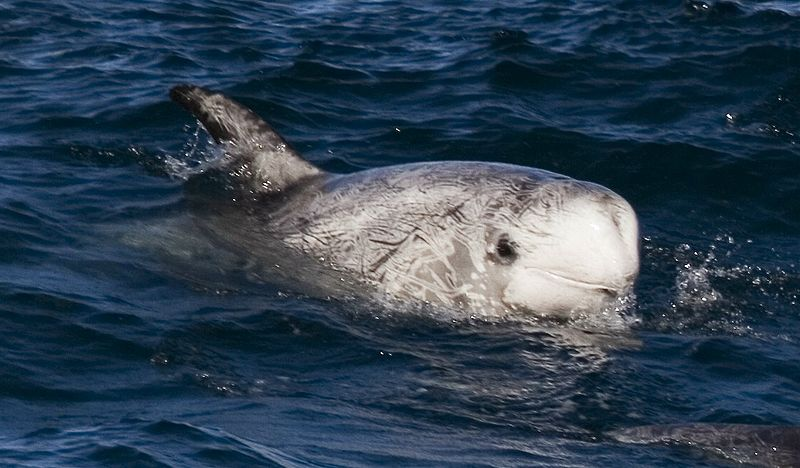
\includegraphics[width=0.65\textwidth]{05/figures/rissosDolphin/rissosDolphin.jpg}  \\
\addvspace{2mm}
\begin{minipage}{\textwidth}
   \caption[rissosDolphinPic]{A Risso's dolphin.\vspace{-1mm} \\
   -----------------------------\vspace{-2mm}\\
   {\footnotesize Photo by Mike Baird (\urlwofont{http://www.bairdphotos.com/}).%Image is under Creative Commons Attribution 2.0 Generic.
}\vspace{-8mm}}
   \label{rissosDolphin}
\end{minipage}
\vspace{3mm}
\end{figure}
\setlength{\captionwidth}{\mycaptionwidth}

Here we identify a confidence interval for the average mercury content in dolphin muscle using a sample of 19 Risso's dolphins from the Taiji area in Japan.\footnote{Taiji was featured in the movie \emph{The Cove}, and it is a significant source of dolphin and whale meat in Japan. Thousands of dolphins pass through the Taiji area annually, and we will assume these 19 dolphins represent a simple random sample from those dolphins. Data reference: Endo T and Haraguchi K. 2009. High mercury levels in hair samples from residents of Taiji, a Japanese whaling town. Marine Pollution Bulletin 60(5):743-747.} The data are summarized in Table~\ref{summaryStatsOfHgInMuscleOfRissosDolphins}. The minimum and maximum observed values can be used to evaluate whether or not there are obvious outliers or skew.

\begin{table}[h]
\centering
\begin{tabular}{ccc cc}
\hline
$n$ & $\bar{x}$ & $s$ & minimum & maximum \\
19   & 4.4	  & 2.3  & 1.7	       & 9.2 \\
\hline
\end{tabular}
\caption{Summary of mercury content in the muscle of 19 Risso's dolphins from the Taiji area. Measurements are in $\mu$g/wet g (micrograms of mercury per wet gram of muscle).}
\label{summaryStatsOfHgInMuscleOfRissosDolphins}
\end{table}

\begin{example}{Are the independence and normality conditions satisfied for this data~set?}
The observations are a simple random sample and consist of less than 10\% of the population, therefore independence is reasonable. The summary statistics in Table~\ref{summaryStatsOfHgInMuscleOfRissosDolphins} do not suggest any skew or outliers; all observations are within 2.5 standard deviations of the mean. Based on this evidence, the normality assumption seems reasonable.
\end{example}

In the normal model, we used $z^{\star}$ and the standard error to determine the width of a confidence interval. We revise the confidence interval formula slightly when using the $t$ distribution:
\begin{eqnarray*}
\bar{x} \ \pm\  t^{\star}_{df}SE
\end{eqnarray*}
\marginpar[\raggedright\vspace{-9mm}

$t^{\star}_{df}$\vspace{1mm}\\\footnotesize Multiplication\\factor for\\$t$ conf. interval]{\raggedright\vspace{-9mm}

$t^{\star}_{df}$\vspace{1mm}\\\footnotesize Multiplication\\factor for\\$t$ conf. interval}The sample mean and estimated standard error are computed just as before ($\bar{x} = 4.4$ and $SE = s/\sqrt{n} = 0.528$). The value $t^{\star}_{df}$ is a cutoff we obtain based on the confidence level and the $t$ distribution with $df$ degrees of freedom. Before determining this cutoff, we will first need the degrees of freedom.

\begin{termBox}{\tBoxTitle{Degrees of freedom for a single sample}
If the sample has $n$ observations and we are examining a single mean, then we use the $t$ distribution with $df=n-1$ degrees of freedom.}
\end{termBox}

In our current example, we should use the $t$ distribution with $df=19-1=18$ degrees of freedom. Then identifying $t_{18}^{\star}$ is similar to how we found $z^{\star}$. 
\begin{itemize}
\setlength{\itemsep}{0mm}
\item For a 95\% confidence interval, we want to find the cutoff $t^{\star}_{18}$ such that 95\% of the $t$ distribution is between -$t^{\star}_{18}$ and $t^{\star}_{18}$.
\item We look in the $t$ table on page~\pageref{tTableSample}, find the column with area totaling 0.05 in the two tails (third column), and then the row with 18 degrees of freedom: $t^{\star}_{18} = 2.10$.
\end{itemize}
Generally the value of $t^{\star}_{df}$ is slightly larger than what we would get under the normal model with~$z^{\star}$.



Finally, we can substitute all our values into the confidence interval equation to create the 95\% confidence interval for the average mercury content in muscles from Risso's dolphins that pass through the Taiji area:
\begin{eqnarray*}
\bar{x} \ \pm\  t^{\star}_{18}SE
	\quad \to \quad
4.4 \ \pm\  2.10 \times 0.528
	\quad \to \quad
(3.29, 5.51)
\end{eqnarray*}
We are 95\% confident the average mercury content of muscles in Risso's dolphins is between 3.29 and 5.51 $\mu$g/wet gram. This is above the Japanese regulation level of 0.4 $\mu$g/wet gram.

\index{data!dolphins and mercury|)}

\begin{termBox}{\tBoxTitle{Finding a $t$ confidence interval for the mean}
Based on a sample of $n$ independent and nearly normal observations, a confidence interval for the population mean is
\begin{eqnarray*}
\bar{x} \ \pm\  t^{\star}_{df}SE
\end{eqnarray*}
where $\bar{x}$ is the sample mean, $t^{\star}_{df}$ corresponds to the confidence level and degrees of freedom, and $SE$ is the standard error as estimated by the sample.}
\end{termBox}

\begin{exercise} \label{croakerWhiteFishPacificExerConditions}
\index{data!white fish and mercury|(}
The FDA's webpage provides some data on mercury content of fish.\footnote{\urlwofont{http://www.fda.gov/food/foodborneillnesscontaminants/metals/ucm115644.htm}} Based on a sample of 15 croaker white fish (Pacific), a sample mean and standard deviation were computed as 0.287 and 0.069 ppm (parts per million), respectively. The 15 observations ranged from 0.18 to 0.41 ppm. We will assume these observations are independent. Based on the summary statistics of the data, do you have any objections to the normality condition of the individual observations?\footnote{There are no obvious outliers; all observations are within 2 standard deviations of the mean. If there is skew, it is not evident. There are no red flags for the normal model based on this (limited) information, and we do not have reason to believe the mercury content is not nearly normal in this type of fish.}
\end{exercise}

\begin{example}{Estimate the standard error of $\bar{x}=0.287$ ppm using the data summaries in Exercise~\ref{croakerWhiteFishPacificExerConditions}. If we are to use the $t$ distribution to create a 90\% confidence interval for the actual mean of the mercury content, identify the degrees of freedom we should use and also find $t^{\star}_{df}$.}
\label{croakerWhiteFishPacificExerSEDFTStar}
The standard error: $SE = \frac{0.069}{\sqrt{15}} = 0.0178$. Degrees of freedom: $df = n - 1 = 14$.

Looking in the column where two tails is 0.100 (for a 90\% confidence interval) and row $df=14$, we identify $t^{\star}_{14} = 1.76$.
\end{example}

\begin{exercise}
Using the results of Exercise~\ref{croakerWhiteFishPacificExerConditions} and Example~\ref{croakerWhiteFishPacificExerSEDFTStar}, compute a 90\% confidence interval for the average mercury content of croaker white fish (Pacific).\footnote{$\bar{x} \ \pm\ t^{\star}_{14} SE \ \to\  0.287 \ \pm\  1.76\times 0.0178\ \to\ (0.256, 0.318)$. We are 90\% confident that the average mercury content of croaker white fish (Pacific) is between 0.256 and 0.318 ppm.}

\index{data!white fish and mercury|)}

\end{exercise}

\subsection{Finding a sample size for a certain margin of error}
\label{findingASampleSizeForACertainME}

\index{margin of error|(}

Many companies are concerned about rising healthcare costs. A company may estimate certain health characteristics of its employees, such as blood pressure, to project its future cost obligations. However, it might be too expensive to measure the blood pressure of every employee at a large company, and the company may choose to take a sample instead.

\begin{example}{Blood pressure oscillates with the beating of the heart, and the systolic pressure is defined as the peak pressure when a person is at rest. The average systolic blood pressure for people in the U.S. is about 130 mmHg with a standard deviation of about 25 mmHg. How large of a sample is necessary to estimate the average systolic blood pressure with a margin of error of 4 mmHg using a 95\% confidence level?}
\label{sampleSizeComputationForSystolicBloodPressure}
First, we frame the problem carefully. Recall that the margin of error is the part we add and subtract from the point estimate when computing a confidence interval. The margin of error for a 95\% confidence interval estimating a mean can be written as
\begin{align*}
ME_{95\%} = 1.96\times SE = 1.96\times\frac{\sigma_{employee}}{\sqrt{n}}
\end{align*}
The challenge in this case is to find the sample size $n$ so that this margin of error is less than or equal to 4, which we write as an inequality:
\begin{align*}
1.96\times \frac{\sigma_{employee}}{\sqrt{n}} \leq 4
\end{align*}
In the above equation we wish to solve for the appropriate value of $n$, but we need a value for $\sigma_{employee}$ before we can proceed. However, we haven't yet collected any data, so we have no direct estimate! Instead, we use the best estimate available to~us: the approximate standard deviation for the U.S. population, 25. To proceed and solve for $n$, we substitute 25 for $\sigma_{employee}$:
\begin{align*}
1.96\times \frac{\sigma_{employee}}{\sqrt{n}} \approx 1.96\times\frac{25}{\sqrt{n}}
	&\leq 4 \\
1.96\times\frac{25}{4} &\leq \sqrt{n} \\
\left(1.96\times\frac{25}{4}\right)^2 &\leq n \\
150.06 &\leq n \\
 n = 151
\end{align*}
The minimum sample size that meets the condition is 151. We round up because the sample size must be \emph{greater than or equal to} 150.06. \Add{and sample size must be an integer}.
\end{example}

A potentially controversial part of Example~\ref{sampleSizeComputationForSystolicBloodPressure} is the use of the U.S. standard deviation for the employee standard deviation. Usually the standard deviation is not known. In such cases, it is reasonable to review scientific literature or market research to make an educated guess about the standard deviation.

\begin{termBox}{\tBoxTitle{Identify a sample size for a particular margin of error}
To estimate the necessary sample size for a maximum margin of error $m$, we set up an equation to represent this relationship:
\begin{align*}
ME = z^{\star}\frac{\sigma}{\sqrt{n}} \leq m 
\end{align*}
where $z^{\star}$ is chosen to correspond to the desired confidence level, and $\sigma$ is the standard deviation associated with the population. Solve for the sample size,~$n$.}
\end{termBox}

Sample size computations are helpful in planning data collection, and they require careful forethought. Next we consider another topic important in planning data collection and setting a sample size: the Type 2 Error rate.

\index{margin of error|)}



\subsection{One sample $t$ tests}
\label{oneSampleTTests}

\index{data!SAT prep company|(}

An SAT preparation company claims that its students' scores improve by over 100 points on average after their course. A consumer group would like to evaluate this claim, and they collect data on a random sample of 30 students who took the class. Each of these students took the SAT before and after taking the company's course, and so we have a difference in scores for each student. We will examine these differences $x_1=57$, $x_2=133$, ..., $x_{30}=140$ as a sample to evaluate the company's claim. 
(This is \emph{paired data}, so we analyze the score differences; for a review of the ideas of paired data, see Section~\ref{pairedData}.) 
The distribution of the differences, shown in Figure~\ref{satImprovementHTDataHistogram}, has mean 135.9 and standard deviation 82.2. Do these data provide convincing evidence to back up the company's claim? 

\begin{figure}[h]
\centering
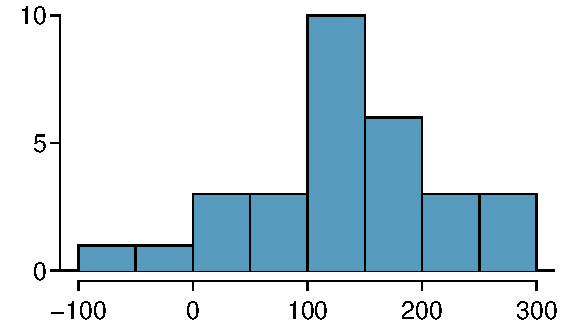
\includegraphics[width=0.54\textwidth]{05/figures/satImprovementHTDataHistogram/satImprovementHTDataHistogram}
\caption{Sample distribution of improvements in SAT scores after taking the SAT course. The distribution is approximately symmetric.}
\label{satImprovementHTDataHistogram}
\end{figure}

\begin{exercise}
Set up hypotheses to evaluate the company's claim. Use $\mu_{_{diff}}$ to represent the true average difference in student scores.\footnote{This is a one-sided test. $H_0$: student scores do not improve by more than 100 after taking the company's course. $\mu_{_{diff}} = 100$ (we always write the null hypothesis with an equality). $H_A$: students scores improve by more than 100 points on average after taking the company's course. $\mu_{_{diff}} > 100$.}
\end{exercise}

\begin{exercise}
Are the conditions to use the $t$ distribution method satisfied?\footnote{This is a random sample from less than 10\% of the company's students (assuming they have more than 300 former students), so the independence condition is reasonable. The normality condition also seems reasonable based on Figure~\ref{satImprovementHTDataHistogram}. We can use the $t$ distribution method. Note that we could use the normal distribution. However, since the sample size ($n=30$) just meets the threshold for reasonably estimating the standard error, it is advisable to use the $t$ distribution.}
\end{exercise}

Just as we did for the normal case, we standardize the sample mean using the Z score to identify the test statistic. However, we will write $T$\index{T score ($T$)|textbf}\marginpar[\raggedright$T$\vspace{0.5mm}\\\footnotesize T score\\(like Z score)]{\raggedright$T$\vspace{0.5mm}\\\footnotesize T score\\(like Z score)} instead of $Z$, because we have a small sample and are basing our inference on the $t$ distribution:
\begin{eqnarray*}
T = \frac{\bar{x} - \text{null value}}{SE} = \frac{135.9 - 100}{82.2/\sqrt{30}} = 2.39
\end{eqnarray*}
If the null hypothesis was true, the test statistic $T$ would follow a $t$ distribution with $df = n-1 = 29$ degrees of freedom. We can draw a picture of this distribution and mark the observed $T$, as in Figure~\ref{pValueShownForSATHTOfOver100PtGain}. The shaded right tail represents the p-value: the probability of observing such strong evidence in favor of the SAT company's claim, if the average student improvement is really only 100.

\begin{figure}
\centering
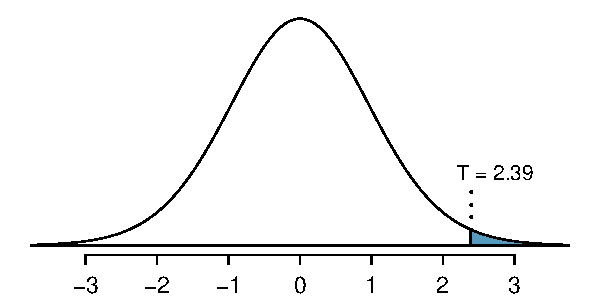
\includegraphics[width=0.65\textwidth]{05/figures/pValueShownForSATHTOfOver100PtGain/pValueShownForSATHTOfOver100PtGain}
\caption{The $t$ distribution with 29 degrees of freedom.}
\label{pValueShownForSATHTOfOver100PtGain}
\end{figure}

\textB{\pagebreak}

\begin{exercise}
Use the $t$ table in Appendix~\vref{tDistributionTable} to identify the p-value. What do you conclude?\footnote{We use the row with 29 degrees of freedom. The value $T=2.39$ falls between the third and fourth columns. Because we are looking for a single tail, this corresponds to a p-value between 0.01 and 0.025. The p-value is guaranteed to be less than 0.05 (the default significance level), so we reject the null hypothesis. The data provide convincing evidence to support the company's claim that student scores improve by more than 100 points following the class.}
\end{exercise}

\begin{exercise}
Because we rejected the null hypothesis, does this mean that taking the company's class improves student scores by more than 100 points on average?\footnote{This is an observational study, so we cannot make this causal conclusion. For instance, maybe SAT test takers tend to improve their score over time even if they don't take a special SAT class, or perhaps only the most motivated students take such SAT courses.}

\index{data!SAT prep company|)}

\end{exercise}

\subsection{Calculator: The 1 sample t-test and CI}

\begin{termBox}{\tBoxTitle{TI calculator: Carrying out the 1 sample t-test}Use \textbf{STAT, TESTS, T-Test}.
\begin{enumerate}
\item Choose STAT.
\item Right arrow to TESTS.
\item Down arrow and choose 8: TInterval.
\item Choose Data if you have all the data or Stats if you have the mean and standard deviation.
\item Let $\mu_0$ be the null or hypothesized value of $\mu$.
\begin{itemize}
\item If you choose Data, let List be L1 or the list in which you entered your data (don't forget to enter the data!) and let Freq be 1. 
\item If you choose Stats, enter the mean, SD, and sample size.
\end{itemize}
\item Choose $\ne$, $<$, or $>$ to correspond to H$_A$.
\item Choose Calculate and hit ENTER.
\begin{description}
\item[] This returns
\end{description}
\begin{tabular}{l l}
\text{t} &\quad \text{t statistic} \\
\text{p} &\quad \text{p-value} \\
$\bar{x}$ &\quad \text{the sample mean} \\
\text{S$_x$} &\quad \text{the sample SD} \\
\text{n} &\quad \text{the sample size}
\end{tabular}
\end{enumerate}
}
\end{termBox}

\begin{termBox}{\tBoxTitle{TI calculator: Calculating the 1 sample t Confidence Interval}Use \textbf{STAT, TESTS, TInterval}.
\begin{enumerate}
\item Choose STAT.
\item Right arrow to TESTS.
\item Down arrow and choose 8: TInterval.
\item Choose Data if you have all the data or Stats if you have the mean and standard deviation.
\item Let $\mu_0$ be the null or hypothesized value of $\mu$.
\begin{itemize}
\item If you choose Data, let List be L1 or the list in which you entered your data (don't forget to enter the data!) and let Freq be 1. 
\item If you choose Stats, enter the mean, SD, and sample size.
\end{itemize}
\item Let C-Level be the desired confidence level.
\item Choose Calculate and hit ENTER.
\begin{description}
\item[] This returns
\end{description}
\begin{tabular}{l l}
\text{( $\_$ , $\_$ )} &\quad \text{the confidence interval} \\
$\bar{x}$ &\quad \text{the sample mean} \\
\text{S}$_x$ &\quad \text{the sample SD} \\
\text{n} &\quad \text{the sample size}
\end{tabular}
\end{enumerate}
}
\end{termBox}

